
\section{Survey}
\label{section:survey}
Through the survey, we aim to make an informed choice when selecting the final agents for the experiment. We provide a range designs that elicit realistic perceptions of intimidation and strength. 

\subsection{Survey Questions}
Participants were told we were interested to see how people perceive traits of avatars based on their design and looks. The goal of evaluating strength and intimidation was not made completely transparent to avoid any possible bias. We gathered demographic data like gender and age. For each avatar, participants had to answer the following questions on a 5-point Likert scale, from 1 --- \textit{Strongly disagree} to 5 --- \textit{Strongly agree}:
\begin{enumerate}
\itemsep0em 
\item This avatar looks attractive.
\item This avatar looks strong.
\item This avatar looks intelligent.
\item This avatar looks intimidating.
\end{enumerate}
We are not interested in measuring intelligence, however it serves the purpose of distracting participants from the specific goal of the survey. Our main interests are strength and intimidation, as these variables may have the effect of changing user performance. Attractiveness is tangentially related because of the Halo Effect \cite{nisbett1977halo}, whereby participants could be determined to assign more positive traits to the avatars. A further consideration with respect to the survey responses is agency. Since social responses can vary with agency \cite{fox2015avatars}, when answering the scale on intimidation, thumbnails of virtual humans may elicit lower responses that actual people.
 
\subsection{Agent Design Coding}
The agents were chosen through stratified sampling to display various levels of strength on a scale from \textit{weak} to \textit{very strong}. In total 36 agents were designed, 18 female and 18 male. The design procedure and implementation for these agents is described in chapter \ref{section:AgentDesign}. Section \ref{subsection:thumbnails} contains an enumeration of the images that users had to rate in this survey and represents the designed look of the agents' upper body. In section \ref{subsubsection:codingTables} we present tables containing a mapping of a unique ID for female (\ref{table:codingFemales}) and male avatars (\ref{table:codingMales}) to an agent design and its respective condition. We use this ID to reference the agent ratings in the following chapters.

\subsection{Participants and Design}
To measure perceived strength in our agent designs, we ran a survey with 31 participants (15 female), aged 21-60 (mean 25.5). Participants were recruited from the university and through snowball sampling. The survey was gender matched and each participant rated 18 avatar thumbnails on a 5-point Likert  scale measuring perceived strength, attractiveness, intelligence and intimidation. The order of the agent thumbnails was the same for all participants, but they were randomly selected from an initial ordered set. The survey took 10 to 15 minutes to complete.

\subsection{Results and Discussion}
\label{section:surveyResults}
Please see section \ref{subsection:thumbnails} for a complete overview of all ratings given to all agents and their respective thumbnail. Tables \ref{tab:f_mean}, \ref{tab:m_mean} from section \ref{subsection:MeanRatings} show the mean ratings given female and males. The tables are ordered ascending according to the \textbf{Weighted} column.


\begin{figure}[H]
\hspace*{\fill}
\centering
\captionsetup{justification=centering,margin=0.1cm}
  \begin{minipage}[b]{0.4\textwidth}
    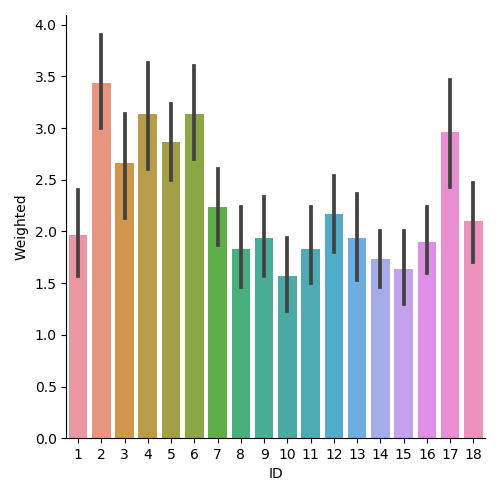
\includegraphics[width=\textwidth]{Survey/weighted_ratings_female_survey.png}
    \caption{Female avatars weighted ratings.}
     \label{fig:SurveyRatedFemalesAll}
    \end{minipage}
\hfill
  \begin{minipage}[b]{0.4\textwidth}
    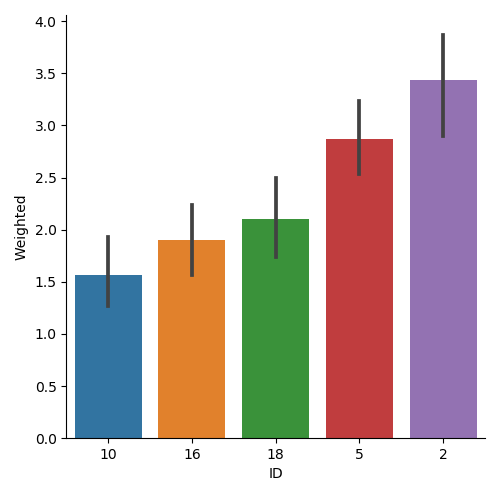
\includegraphics[width=\textwidth]{Survey/weighted_ratings_female_survey_chosen.png}
    \caption{Chosen female avatars weighted ratings.}
     \label{fig:SurveyRatedFemalesChosen}
  \end{minipage}
\hspace*{\fill}
\end{figure}
\begin{figure}[H]
\hspace*{\fill}
\centering
\captionsetup{justification=centering,margin=0.1cm}
  \begin{minipage}[b]{0.4\textwidth}
    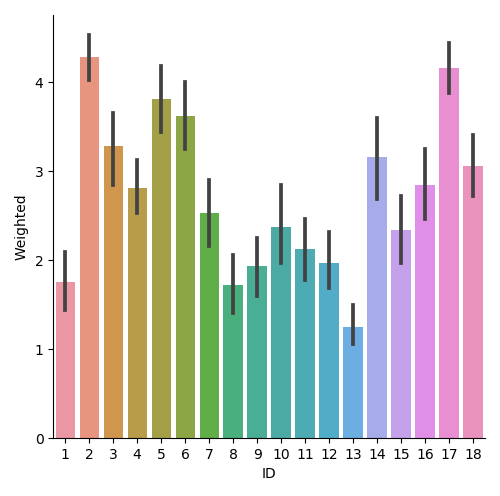
\includegraphics[width=\textwidth]{Survey/weighted_ratings_male_survey.png}
    \caption{Male avatars weighted ratings.}
     \label{fig:SurveyRatedMmalesAll}
    \end{minipage}
\hfill
  \begin{minipage}[b]{0.4\textwidth}
    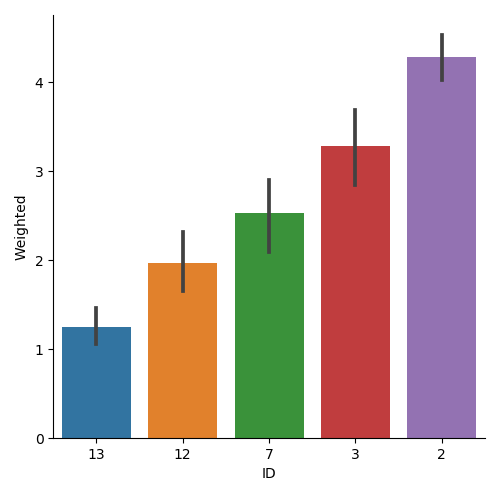
\includegraphics[width=\textwidth]{Survey/weighted_ratings_male_survey_chosen.png}
    \caption{Chosen male avatars weighted ratings.}
     \label{fig:SurveyRatedMalesChosen}
  \end{minipage}
\hspace*{\fill}
\end{figure}

To determine the final avatars for the user study, we compounded the strength and intimidation rating and computed a final weighted score according to the following formula: $ 0.5 strength + 0.5 intimidation $. This value can be found in the \textbf{Weighted} column. 
As a reference for the other chapters, the chosen UMAs are marked in the table in the \textbf{UMA} column. The first part of the column value represents a unique identifier for the UMA design and the second part is the condition shorthand, where C1 denotes the weak condition, C2 average and C3 strong. The unique identifier is shown on the x axis in the above table as ID.
Users generally found UMA designs unattractive. Female ratings for intimidation and strength were lower than male ones.
\\
As expected, female ratings were overall lower than male ratings. This is a limitation of the UMA DNA ranges and difference in character enhancements magnitude between  genders and races. Female upper and lower body muscle mass could be increased less than for males. Males had more defined muscle, while for female muscle tone decreased with muscle mass. Other downsides of increasing body mass for females was that leg muscles grew non-uniformly and appeared unnatural. Some other disadvantages are mentioned in the previous chapter. We consider the Morph Character System (MCS) as an alternative to UMA, however support for current Unity versions has been discontinued for this library.

\subsection{Conclusion and Improvements}
For more control over avatar variation, we can consider a custom design for the avatars using a 3D modelling tools.  UMA has the advantage of providing a simplified and fast method of generating many avatars with some degree of control over the body-related changes. Conversely, 3D tools are have a high learning curve and can be difficult for inexperienced users. To allow the same magnitude of change for all body modifications, we would ideally implement a VR character creator with a simple user interface. With respect to appearance modification, other body enhancements such as piercings ca be considered.
